\documentclass[tikz,border=7pt]{standalone}
\usepackage{amsmath}
\usetikzlibrary{arrows.meta}

\definecolor{ink}{HTML}{21352F}
\definecolor{teal}{HTML}{087F7B}
\definecolor{rose}{HTML}{B65A62}
\definecolor{gold}{HTML}{C58B2A}
\definecolor{blue}{HTML}{4B77A8}

\begin{document}
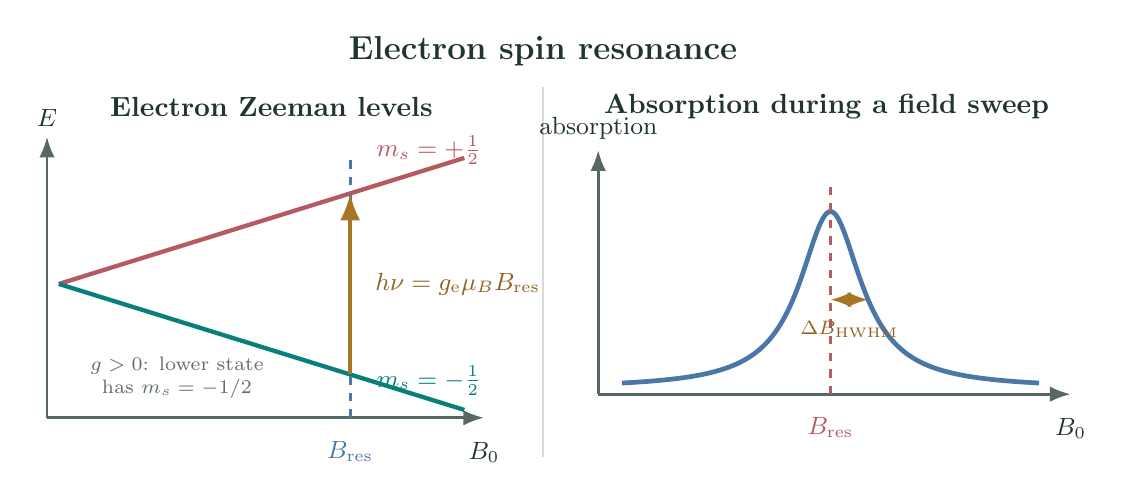
\begin{tikzpicture}[font=\sffamily,>=Latex]
  \node[font=\bfseries\large,text=ink] at (0,2.8)
    {Electron spin resonance};

  % Zeeman level diagram, E = g mu_B B m_s.
  \node[font=\bfseries,text=ink] at (-3.45,2.1)
    {Electron Zeeman levels};
  \draw[->,line width=1pt,draw=ink!75]
    (-6.3,-1.85) -- (-0.75,-1.85)
    node[below=5pt,text=ink,font=\small] {$B_0$};
  \draw[->,line width=1pt,draw=ink!75]
    (-6.3,-1.85) -- (-6.3,1.72)
    node[above,text=ink,font=\small] {$E$};

  \draw[line width=1.55pt,draw=rose]
    (-6.15,-0.15) -- (-1.0,1.45);
  \draw[line width=1.55pt,draw=teal]
    (-6.15,-0.15) -- (-1.0,-1.75);
  \node[text=rose,font=\small] at (-1.45,1.55) {$m_s=+\tfrac12$};
  \node[text=teal,font=\small] at (-1.45,-1.38) {$m_s=-\tfrac12$};

  \draw[dashed,line width=1pt,draw=blue]
    (-2.45,-1.85) -- (-2.45,1.45);
  \node[below=5pt,text=blue,font=\small] at (-2.45,-1.85)
    {$B_{\mathrm{res}}$};
  \draw[->,line width=1.5pt,draw=gold!85!black]
    (-2.45,-1.30) -- (-2.45,1.00)
    node[midway,right=5pt,text=gold!72!black,font=\small]
    {$h\nu=g_{\mathrm e}\mu_BB_{\mathrm{res}}$};
  \node[text=ink!72,font=\scriptsize,align=center] at (-4.65,-1.34)
    {$g>0$: lower state\\has $m_s=-1/2$};

  \draw[ink!18,line width=1pt] (0,-2.35) -- (0,2.35);

  % Fixed-frequency field sweep.
  \node[font=\bfseries,text=ink] at (3.6,2.1)
    {Absorption during a field sweep};
  \draw[->,line width=1pt,draw=ink!75]
    (0.7,-1.55) -- (6.7,-1.55)
    node[below=5pt,text=ink,font=\small] {$B_0$};
  \draw[->,line width=1pt,draw=ink!75]
    (0.7,-1.55) -- (0.7,1.55)
    node[above,text=ink,font=\small] {absorption};

  % Lorentzian centered at B_res.
  \draw[line width=1.7pt,draw=blue,domain=-2.65:2.65,samples=140,smooth,
        variable=\x]
    plot ({3.65+\x},{-1.48+2.25/(1+(\x/0.48)^2)});
  \draw[dashed,line width=1pt,draw=rose] (3.65,-1.55) -- (3.65,1.08);
  \node[below=5pt,text=rose,font=\small] at (3.65,-1.55)
    {$B_{\mathrm{res}}$};
  \draw[<->,line width=1pt,draw=gold!85!black]
    (3.65,-0.35) -- (4.13,-0.35)
    node[midway,below=4pt,text=gold!72!black,font=\scriptsize]
    {$\Delta B_{\mathrm{HWHM}}$};
\end{tikzpicture}
\end{document}
